\documentclass[UTF8,a4paper,11pt,fontset=fandol]{ctexart}
\usepackage[margin=2.15cm]{geometry}
\usepackage{booktabs,tabularx,array,amsmath,graphicx,caption,fancyhdr,enumitem,xcolor,hyperref}
\hypersetup{hidelinks,pdfauthor={钱森}}
\pagestyle{fancy}\fancyhf{}\fancyfoot[R]{\thepage}\renewcommand{\headrulewidth}{0pt}
\setlength{\parskip}{3pt}\setlength{\emergencystretch}{2em}
\setlist{nosep,leftmargin=2em}
\newcommand{\titleline}[1]{\begin{center}{\LARGE\bfseries #1}\par\vspace{5pt}钱森\end{center}}
\newcommand{\fn}[1]{\nolinkurl{#1}}
\newcolumntype{L}{>{\raggedright\arraybackslash}X}


\usepackage{float}
\begin{document}
\titleline{青河流域洪水预报系统二期实践报告}
\begin{abstract}
第二场洪水的基准预报峰值为868.59\,m³/s，距青河水文站保证阈值仅31.41\,m³/s。围绕这次临界预报，二期系统把一期新安江引擎接入资料质控、版本化起报、情景计算、站内预警和产品签发流程。保持初始状态与参数相同，仅将雨量增加10\%，原雨型下的洪峰即升至1054.29\,m³/s。引入实时观测后，第四场的均方根误差略有下降，前三场均有上升；第二场峰后一个时段的误差反向解释了其中最显著的增幅。系统将签发依据与结果一并冻结，既能追溯当时采用的方案，也能在观测更新、参数归档和服务重启后复算原产品。
\end{abstract}

\section{从出口流量到预报公报}
以第二场洪水为例，值班员面对三个连续的判断：基准过程达到哪一级阈值？若降雨偏强或提前到来，等级是否会改变？复核人员随后拿到的公报，是否对应值班员看到的那次计算？第一个问题需要一条可信的流量过程，第二个问题需要在相同条件下改变降雨，第三个问题则要求保存计算发生时的数据和参数。这三个判断贯穿本次系统设计与验收。

青河教学流域面积2000\,km²，数据由四场洪水组成，每场40个6小时时段。六站雨量按泰森权重汇总为面雨量，蒸发皿记录转换为时段蒸发能力。一期模型完成蒸散发、蓄满产流、三水源划分及汇流，再通过马斯京根河道演算输出青河水文站流量。二期沿用前三场率定后冻结的16个参数，以第四场检验移植精度。四场160个基线流量点与一期归档曲线的最大绝对差为 $3.41\times10^{-13}$\,m³/s。由此，后文比较降雨情景和滚动校正时，可以把差异定位到具体改变的输入或状态。

\section{哪些资料可以起报}
不同缺测对计算的影响不同。雨量和蒸发进入水量计算，少一个站点雨量就无法沿用既定六站权重。出口观测主要用于过程对比和状态更新，某一时段缺测，模型仍有足够的强迫数据继续演算。系统按字段保存行号、异常原因和严重程度，并把这一区别落实到起报条件中。
\begin{table}[H]\centering\small\caption{用第一场资料验证两类异常的处理}
\begin{tabularx}{\linewidth}{@{}p{.28\linewidth}LL@{}}\toprule 输入变化 & 入库后的处置 & 起报与评价结果\\\midrule
首时段出口观测置为缺测标记 $-999$ & 保留该时段，观测记为空，登记警告 & 完成40步演算，缺测步跳过同化，精度采用39个有效观测。\\
首个站点雨量改为 $-2$\,mm，另复制一行造成重复时刻 & 标出异常字段和不符合6\,h间隔的时刻 & 场次标为阻断，起报返回质控错误，可据行列修正后重新导入。\\\bottomrule\end{tabularx}\end{table}
每场资料还包含三层土壤蓄水、自由水蓄量以及三个水源的初始出流。导入新场次时须提供这七项初值。参数方案需包含完整的16个参数，河道传播参数满足 $2KE X\le6\le2KE(1-X)$，使6\,h递推系数非负。资料和方案均通过检查后，手动起报与定时起报进入同一个计算入口。

\section{一次起报如何固定版本并完成签发}
\subsection{输入、计算与结果的边界}
浏览器和周期调度器通过同一应用服务提交起报请求。FastAPI 检查请求字段，应用服务在一次数据库读取事务中取得场次和指定方案；若请求未指定版本，则读取该时刻的活动版本。快照保存标准化时序、初始状态、参数实值、情景和阈值，还保存原始文件及引擎的摘要。模型随后使用这份快照计算。这样，即使下一位值班员在计算期间切换方案，同一条曲线的前后时段仍使用同一组参数。

结果入库时，系统在同一写事务内登记草稿、起报审计和相应的超警消息。工作台在收到新消息后显示未读提示，值班员可沿消息中的预报编号打开对应过程线。预警在起报成功时产生，正式公报则需复核人员显式签发，两项操作的时机不同。周期任务同样先生成草稿。系统保存下次到期时刻、最近运行编号和错误信息，重启后从持久化的调度记录继续工作。

\begin{figure}[H]\centering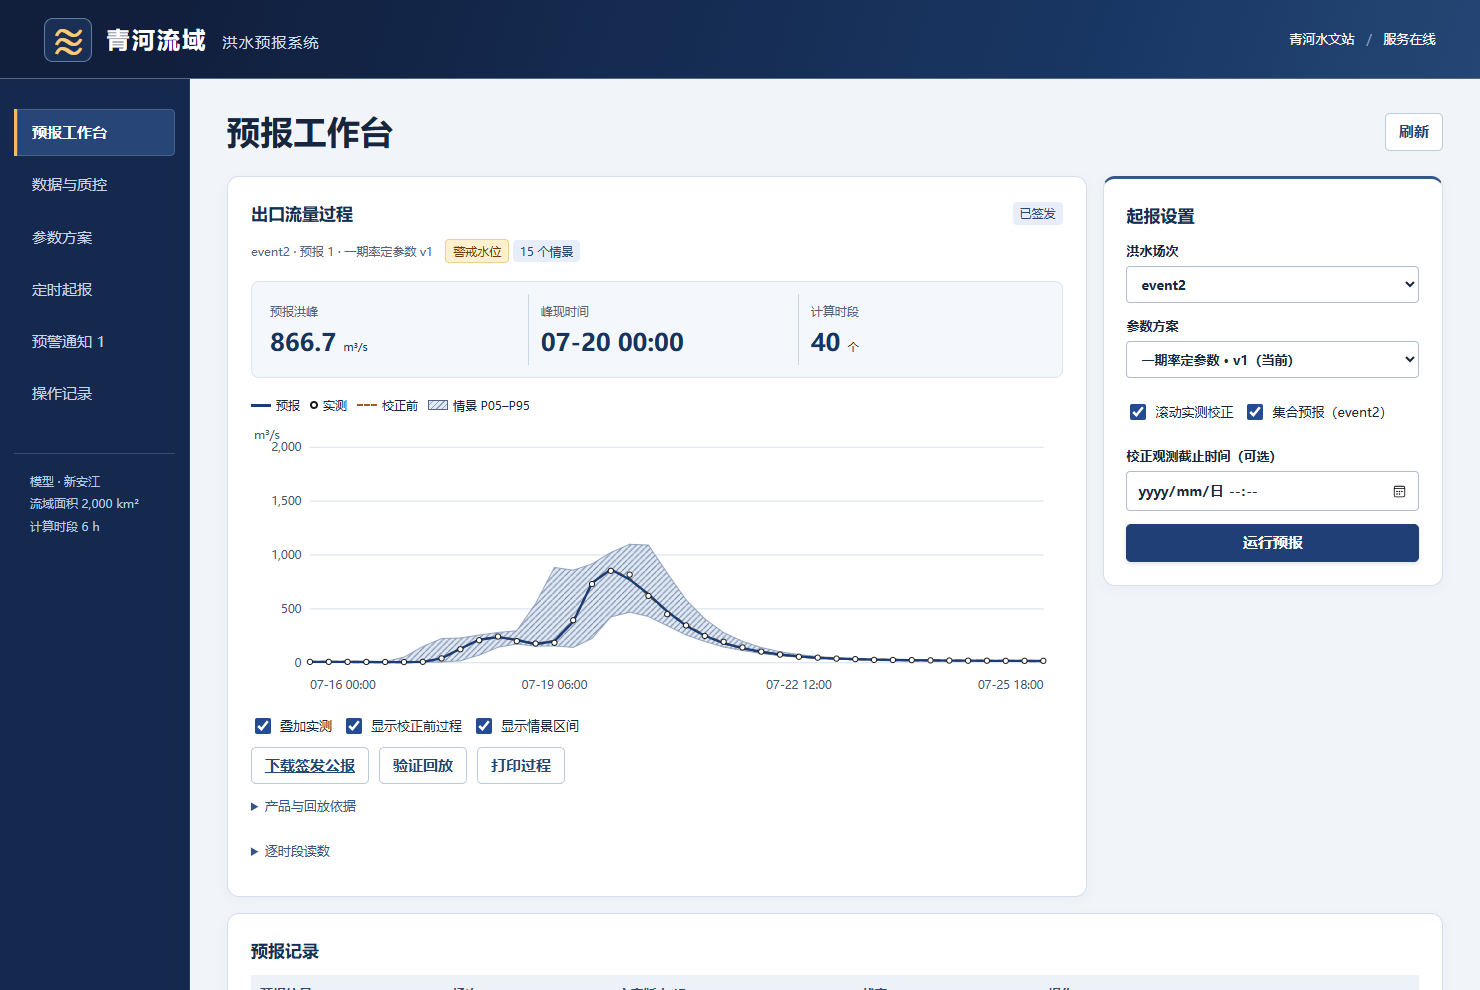
\includegraphics[width=.96\linewidth]{figures/workbench.png}
\caption{第二场洪水的签发界面。右侧选择方案与计算选项，左侧核对观测、预报及分位带。本次浏览器演示开启校正，显示洪峰866.7\,m³/s。}\end{figure}
\subsection{以归档公报核对产品}
归档样例 \fn{QH-00000001} 来自另一次关闭校正的基准起报。它给出的峰时为7月20日00时，峰值868.59\,m³/s，等级为警戒，附7月16日00时至7月25日18时的40个时段和流量单位。两次起报分别保存校正开关，因此样例与图1所示产品可以按各自的设置解释。签发前访问公报下载接口返回409；首次签发后保存签发人和时间，重复点击仍保留首次记录。下载文件含快照与结果的 SHA-256 摘要，可用于核对归档内容。

\section{越警判断对降雨假设有多敏感}
第二场的基准洪峰比警戒值500\,m³/s高368.59\,m³/s，而与保证值900\,m³/s只差31.41\,m³/s。为了判断这一级差对降雨假设的敏感程度，固定模型、参数、初始蓄水与蒸发，关闭实时校正。将每站雨量乘以0.8、0.9、1.0、1.1、1.2五种倍率，再分别前移12\,h、保持原位和后移12\,h。窗口外的雨量移出，移入端补零。计算器以最多四个工作线程运行15个成员。
\begin{figure}[H]\centering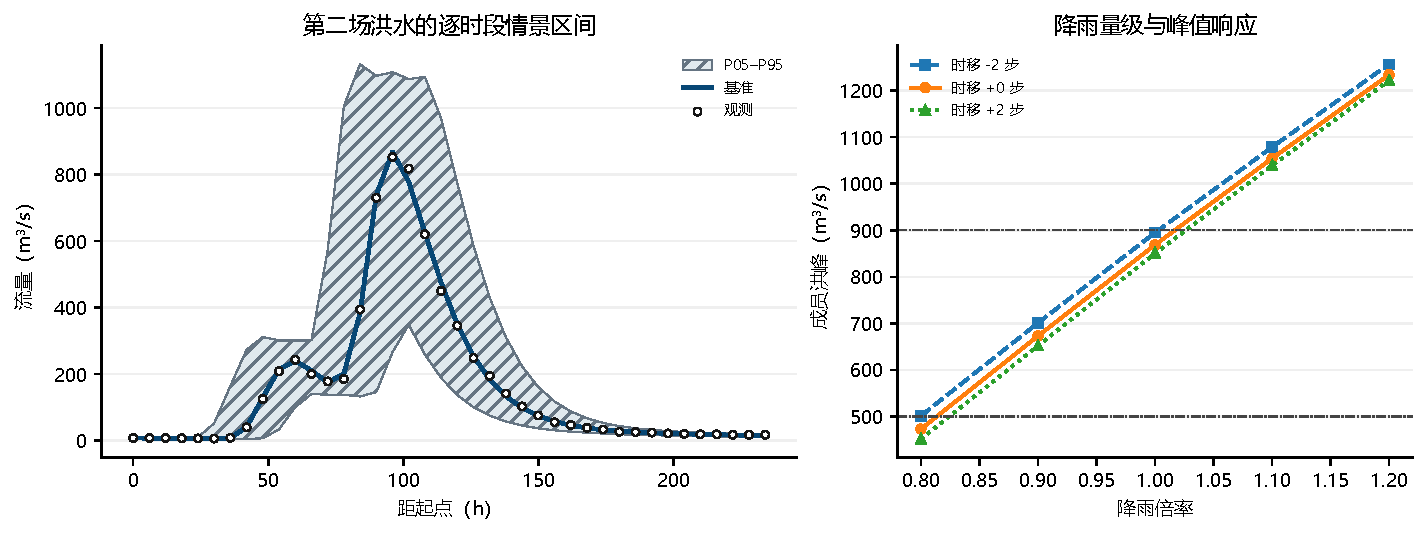
\includegraphics[width=\linewidth]{figures/ensemble.pdf}
\caption{第二场降雨扰动试验。左图对每个时段的15个流量取分位数，右图对每条成员曲线分别取峰值。两种统计量回答不同的问题。}\end{figure}
\textbf{雨量幅度改变了预警等级。}保持原雨型，倍率由1.0增至1.1，洪峰从868.59升至1054.29\,m³/s，增加185.69\,m³/s；1.1倍率组的三个时移都达到保证阈值。在0.8倍率组，原位的洪峰为473.07\,m³/s，提前12\,h后为501.44\,m³/s，刚好跨过警戒值。只报告雨量倍率，会漏掉这个由降雨时序引起的等级变化。

\textbf{判断越限应逐成员取峰。}在基准峰时7月20日00时，15个成员的中位流量为619.58\,m³/s，明显低于基准曲线的868.59\,m³/s。原因是扰动改变了各成员到峰的时刻。统计整个过程时，13个成员的洪峰达到警戒值，其中6个达到保证值。签发时可以据此写明“基准为警戒，偏强降雨情景达到保证值”。15个组合是等权设计情景，$6/15$描述这组试验的越限频数。工作台保留逐时段 P05、P50、P95，供复核人在不同时间查看流量范围。

\section{滚动校正的收益与代价}
\subsection{一条观测在什么时刻起作用}
设$Q_t^-$为本时段发布的先验流量，$y_t$为当时已收到的观测。系统先发布$Q_t^-$，再以固定增益0.5修正供下一时段使用的河道出流状态：
\[
Q_t^+=Q_t^-+0.5(y_t-Q_t^-).
\]
没有有效观测或已超过用户指定的截止时刻时，取$Q_t^+=Q_t^-$。同一组河道入流下，设$B_t$为未校正流量，则下一时段相对基线的变化满足
\[
 Q_{t+1}^--B_{t+1}=c_2(Q_t^+-B_t),\qquad
 c_2=\frac{KE(1-X)-\Delta t/2}{KE(1-X)+\Delta t/2}=0.5807 .
\]
因此，当前观测的影响至少相隔一个6\,h时段才出现在预报曲线上。追加观测后再次起报，早先签发的快照仍保留原来的可用观测和截止时刻。

\textbf{截止时刻的验证。}用第二场数据做一次只改观测的对照，取第13个时段为截止点。将该点的观测增加80\,m³/s，前13步发布值逐点相同，基线也完全相同。按递推式，截止点更新后的状态比原状态高40\,m³/s，下一步发布值应增加约23.23\,m³/s。再将截止点之后第二个时段的观测增加200\,m³/s，得到的整条预报曲线与前一次相同。这项检验把“能够吸收新观测”和“不会提前使用未来观测”分别落实到可检查的时段上。

\subsection{为什么同一增益在四场洪水上表现不同}
\begin{table}[H]\centering\small\caption{同一场资料在开关滚动校正时的比较。两组共用强迫、初始状态和参数，RMSE单位为 m³/s。}
\begin{tabular}{lrrrr}\toprule 场次 & 基线 DC & 滚动 DC & 基线 RMSE & 滚动 RMSE\\\midrule
event1 & 0.999734 & 0.999698 & 1.225565 & 1.304307 \\
event2 & 0.998397 & 0.998015 & 9.131170 & 10.162790 \\
event3 & 0.999730 & 0.999658 & 3.011953 & 3.391430 \\
event4 & 0.999085 & 0.999108 & 3.444164 & 3.400310 \\
\bottomrule\end{tabular}\end{table}
第四场的RMSE从3.444降至3.400\,m³/s，前三场均升高，第二场增幅最大。可从第二场洪峰过后的两步直接看到这一差异如何形成。
\begin{table}[H]\centering\small\caption{第二场转入退水时的逐步校正。残差取预报减观测，各列单位为 m³/s。}
\begin{tabular}{lrrrrr}\toprule 7月20日 & 观测 & 基线 & 滚动预报 & 基线残差 & 滚动残差\\\midrule
00时 &853.10&868.59&866.69&$+15.49$&$+13.59$\\
06时 &818.00&778.94&773.89&$-39.06$&$-44.11$\\
12时 &620.80&626.13&636.00&$+5.33$&$+15.20$\\\bottomrule\end{tabular}\end{table}

00时，滚动预报比观测高13.59\,m³/s，更新把状态向下拉。到06时，基线本已低估39.06\,m³/s，上一步的状态修正又把预报压低5.05\,m³/s，使该时段平方误差增加420.25\,(m³/s)$^2$，约占整场净增量796.16的52.8\%。06时观测高于模型，状态随即上调；到12时，基线误差已再次变为正值，上调又扩大了高估。峰区误差连续反向，使固定增益在这一场付出了较大的滞后代价。

第四场的改善也有时段差异。8月30日06时，滚动校正把峰区高估从12.73缩小到11.29\,m³/s；12时基线已经低估，校正又把误差从$-8.01$扩大到$-12.13$\,m³/s。把40步平方误差逐一相减再求和，全场净减少12.01\,(m³/s)$^2$。四场数据支持在工作台保留两条曲线，让复核人结合近期残差方向使用校正结果。

\section{历史产品如何复核}
回放读取签发时的输入和参数，先核对快照与已存结果的摘要，再核对计算引擎版本。重算后的摘要与原结果一致，才返回回放成功。为检验历史产品是否真的独立于当前数据库配置，测试先建立同名方案两个版本，将蒸发折算系数分别设为0.90和0.95。用第一版对第二场起报，随后启用第二版、归档第一版，并重新导入上层初始蓄水改为0的场次。此时旧编号仍可回放得到相同摘要，新起报则得到不同摘要。这一对照同时覆盖了方案切换、旧版归档和原始场次更新。

公报归档时保留两种摘要，各有不同用途。以第二场样例为例，快照摘要以 \texttt{ed6f7501} 开头，用于核对当时的资料、参数与设置；结果摘要以 \texttt{5aae3999} 开头，用于核对基准过程、情景及评价结果。引擎源码经统一编码和换行后计算版本指纹，回放时先检查指纹，再执行数值计算。这使 Windows 开发机与 Linux 容器之间单纯的换行差异不会被误判为模型升级。

\subsection{交付验收覆盖了哪些运行边界}
真实浏览器从 CSV 上传与质控开始，完成了集合起报、消息已读、签发公报下载及历史回放。对于浏览器界面无法观察到的数据持久性，另安排了以下三项检查。
\begin{table}[H]\centering\small\caption{对同一预报编号的三种核验}
\begin{tabularx}{\linewidth}{@{}p{.18\linewidth}LL@{}}\toprule 验收环节 & 操作 & 可检查的结果\\\midrule
重复签发 & 同一草稿由第一位复核人签发，再用另一署名提交同一请求 & 原签发人及时间保持一致，审计中签发动作只出现一次。\\
容器重启 & 保存签发编号和结果摘要，重启服务并重新连接数据库 & 原编号仍为已签发，读取的结果摘要相同，快照重算匹配。\\
独立副本恢复 & 对运行中的数据库做在线备份，在新文件上创建服务，并按编号回放 & 副本可读出原签发产品；快照、结果摘要均与原库相同。\\\bottomrule\end{tabularx}\end{table}

四场黄金序列随代码固定保存；滚动校正诊断另存160行数据，每行列出观测、基线、滚动值及平方误差增减量，可直接复算表中结果。19项自动化测试通过，接口契约、容器构建、签发与重启回放随提交在持续集成中重新验证。

\section*{结论}
第二场预报给出了两项不同的值班依据：按当前降雨与参数应发出警戒通知，按偏强降雨准备复核保证阈值。滚动校正则需要结合观测时效和峰区误差方向判断，观测到达越及时，并不必然使下一步流量越准确。系统把选定的降雨、参数版本、观测截止时刻及计算结果随编号保存，使上述判断在签发时有据可查，在资料更新后也可复算。
\end{document}
